\section{Experiments}
\vspace{-0.3cm}
\label{sec:applications}
% This section presents experiments which exemplify the CC properties discussed  in Sec.~\ref{sec:features}. It further proposes potential use-cases of CC in various Computer Vision applications.

\textbf{Visualizing the continuous learned kernels $K_\theta$:} Filters of discrete conv-layers can be easily visualized. They are sets of discrete numbers on a regular grid, which can just be printed out or viewed as images. Filters of CC-layers, on the other hand, assign a unique set of numbers to any sub-`pixel' grid location. But once trained,
%the Internal-Net $K_\theta$ is trained, 
we can easily sample $K_\theta$ on a regular grid at any desired resolution for the purpose of visualization. Fig.~\ref{fig:visualize} shows 2 such examples of CC kernel visualization. In both examples we trained a single CC-layer to \emph{imitate} an image-resizing method (for which we know the ground-truth kernels): (i) Imitate bicubic resizing, and (ii) imitate resizing by a Gaussian kernel with different $\sigma$ for each axis, rotated by~\ang{45}.  The CC-training was performed  on a single image with a single random sampled scale $s$$\in$$[0.3$$,..,$$1.3]$ in each dimension. The input to the CC-layer was the single image, and the ``output label'' was the resized image  (generated by the external image-resizing method for that $s$).  
%We tested it for: (i)~the well known bicubic resizing; and (ii) a non-isotropic interpolation method -- a Gaussian with different $\sigma$ for each axis, rotated by~\ang{45}. 
Once trained, we sampled $K_\theta$ at dense 200$\times$200 coordinate-pairs.  Fig.~\ref{fig:visualize} shows such visualizations of the  continuous recovered kernel $K_\theta$,  as a function of the training iteration.
%, showing good convergence to the correct ground-truth continuous kernel.

\textbf{Verifying  scale generalization:} To test generalization across scales, we sampled a \emph{single}  pair of random scale-factors $s_x$,$s_y$$\in$$[0.3$$,..,$$1.3]$, and applied an independent bicubic resizing to a single image for this scale. As before, we trained a CC-layer with the original image as  the input, and the resized image as the ``output label''. To test generalization, we applied our CC-layer  (which was {trained} for one scale), on 100 \emph{new random scales}. We compared the resulting 100 output images to ground-truth bicubic resizing by those 100 scales. The left side of Fig.~\ref{fig:generalize} shows  MSE of the train-error and the generalization (test) error. The test-error for scales CC never trained for, is very close to the train-error for the single scale it trained on. This is due to the fact that CC generalizes well to other scales, as long as the training scale generates sufficient diversity in sub-`pixel' grid shifts. To further confirm this, we repeated the experiment, only this time we chose the training scale to be $1/int$ (1/2). Eq.~\ref{eq:grid} shows that in such case all grid locations have the same shift from `pixel' centers (0.5). The right side of Fig.~\ref{fig:generalize} shows that generalization was severely damaged; test-error for 100 other scales was 2-orders-of-magnitude higher. Fig.~\ref{fig:generalize} further shows visualization of $\mathcal{K}_\theta$ for these 2 experiments (ground-truth can be found in Fig.~\ref{fig:visualize}). In the first experiment the learned kernel is similar to the ground-truth, whereas in the second experiment it
is not (since it was only required to produce correct results for a very small subset of coordinate pairs).



% \textbf{Exploiting CC for image classification -- the power of dynamic Scale-Ensembles at inference time:}
% To demonstrate the potential use of CC-layers in
% %that replacing standard conv-layers by CC-layers may improve 
% image classification tasks, we did the following simple experiment:
% We used a variant of a very simple CNN-based classification net for CIFAR-10~\cite{CIFAR10} (similar to the net used in~\cite{wong2018scaling, atzmon2019controlling}). The network consisted of several conv-layers of strides 1,2,1,1,1,2, followed by 3 fully-connected layers, all with ReLU activations. We call this the ``Baseline Net''.

% We construct a ``CC-Classifier'' 
% with the same number of layers, but with CC-layers of \emph{gradually} changing scale factors (starting from the second layer), so that the overall scale factor from the net's input to the last conv-layer's output remains the same (1:4).  
% %At each training iteration a sequence of scale-factors whose \emph{product} yields the global scale factor $\nicefrac{1}{4}$ is randomly sampled  (as in Fig.~\ref{fig:scale_ensemble}). 
% A sequence of scale-factors whose \emph{product} yields the global scale factor $\nicefrac{1}{4}$ is randomly sampled for training the network. 
% %
% %The resulting network gave a pronounced improvement in classification accuracy (+1.4\%).
% %To isolate the impact of the higher number of params in our CC-layers, we further tested a ``CC-baseline'' classifier, which has the same integer scales and strides as in the regular Baseline-Net.
% %All 3 networks were trained in parallel, on same batches with same conditions.
% Both  networks were trained in parallel, on same batches with same conditions.

% Note that since our gradual  ``CC-classifier'' was trained with non-integer (float) scale-factors, it can generalize to any new intermediate scale-factors \emph{at inference-time}. This gives rise to \emph{ensemble-based image classification} (see Sec.~\ref{sec:features} and Fig.~\ref{fig:scale_ensemble}). 
% We tested with varying numbers of scale-ensembles (0, 2, 5). \ben{0?}
% Our CC-classifier gave a pronounced  improvement in classification accuracy compared to the Baseline-Net, which grew with the number of scale-ensembles (+0.4\%, 2\%, 2.2\%, respectively). 

% For fair comparison we performed two extra tests:
% (i)~Scale-ensembles can be regarded as test-time `augmentations'. Hence, we also provided test-time augmentations to the Baseline-Net, by augmenting input images with mild scale variations and horizontal-flip. The predicted class was the argmax of the averaged logits.
% %we used mild random scaling (scale-factor between 1 and 1.1) and center-cropping of the input image. We observed that scaling hardly improves their results so we also used horizontal flips for both our test-augmentations and for the baselines.
% Such augmentations gave a slight improvement (up to +0.86\% for 5 augmentations), but not as significant as the scale-ensembles (+2.2\% for 5 ensembles). \ben{not 5 ensembles. maybe ensemble of 5?}
% (ii)~To isolate the impact of the higher number of params in our CC-layers, we further tested a ``CC-baseline'' classifier with CC-layers (same number of params as the ``CC-Classifier''), but with the same integer scales \& strides as in the ``Baseline-Net''. Indeed, the extra number of params proved to be a major factor in improved performance when no ensembles/augmentations were used (might also be due to using the accurate grid projection of Eq.~\ref{eq:grid}, used by both CC-Classifier and CC-Baseline \ben{I think that's not true. the cc-layers in base-cc are equivalent to conv-layers in terms of expressiveness. that is, one can choose weights for base that would make it exactly the same as a given base-cc network}). However, since the CC-Basline was trained on integer scale-factors, it cannot generalize to new scales at test-time, hence cannot employ scale-ensembles at inference time (only regular image augmentations, which gave at best +0.55\% to the CC-baseline). As mentioned above, the scale-ensembles gave the most significant boost in classification performance. \emph{This new inference-time capability can  be achieved only with CC-Classifiers.} \ben{question: do we have the result of cc-classifier with the same 5 augmentations as base and base-cc? if so, was it good? bad?}


% \michal{Shall we show a comparison also to feature interpolation methods?}


% % Table.~\ref{table:res} shows the accuracy over the test-set of CIFAR-10. For each method we specify the results for several numbers of test-augmentations. The best result for each method across number of test-augmentaions is underlined. The overall best score is in bold. CC based networks achieve higher accuracy with margin that grows along the depth of the networks. For the deeper networks, we see that scale-augmented CC outperforms the base CC.


% % \textbf{Scales ensemble for image classification:}
% % To demonstrate scales ensemble we tested classification of CIFAR-10 \cite{CIFAR10}. As a baseline we used a simple CNN based on the one used in \cite{wong2018scaling, atzmon2019controlling}. The network consists of 4 of conv-layers of strides 1, 2, 1, 2 respectively and then 3 fully-connected layers. All with ReLU activations. To characterize the effect of depth, we also used variants of the network, by adding various numbers of stride-1 conv-layers before the last stride-2 layer. 
% % The CC based Classifier, has the same number of layers, but with changing scale factors, starting from the second layer. At each iteration a set of scale factors with multiplication of $\nicefrac{1}{4}$ is sampled randomly, as in Fig.~\ref{fig:scale_ensemble}. We also tested a CC based classifier, but with constant strides, same as in the baseline- Base CC, that has the same number of parameters.Training was done in parallel, so that all networks trained exactly on the same batches with the same conditions.

% % We demonstrated the results of the CC classifier when ensembling various number of test-augmentations. However, for fair comparison we used self-ensemble for the base-lines too. Since their intermediate layers cannot be rescaled, we used mild random scaling (scale-factor between 1 and 1.1) and center-cropping of the input image. We observed that scaling hardly improves their results so we also used horizontal flips for both our test-augmentations and for the baselines.

% % Table.~\ref{table:res} shows the accuracy over the test-set of CIFAR-10. For each method we specify the results for several numbers of test-augmentations. The best result for each method across number of test-augmentaions is underlined. The overall best score is in bold. CC based networks achieve higher accuracy with margin that grows along the depth of the networks. For the deeper networks, we see that scale-augmented CC outperforms the base CC.


\textbf{Verifying Shift-Equivariance:}
To check shift-equivariance, we used a variant of a very simple CNN-based classification net for CIFAR-10~\cite{CIFAR10} (similar to the net used in~\cite{wong2018scaling, atzmon2019controlling}). The network consisted of several conv-layers of strides 1,2,1,1,1,1,1,2, followed by 3 fully-connected layers, all with ReLU activations. We call this the ``Baseline Net''.
%
We constructed a ``CC-Net'' 
with the same number of layers, but with CC-layers of \emph{gradually} changing layer sizes (starting from the second layer). The overall scale factor from the net's input to the last conv-layer's output remained the same (1:4), and the scale-factors of all layers were approximately ${(\nicefrac{1}{4})^{\nicefrac{1}{6}}}$. When testing on the CIFAR-10 test-set, CC-Net had higher accuracy (87.81\%) compared to the Baseline (87.14\%), which is not surprising as CC-Net has more params than Baseline-Net, but was not the purpose of this experiment. 
%5When applying scale ensemble of 5 scale-sequences, CC-Net climbed to 90.19\%.
%For the equivariance test no self-ensemble of any kind was used for neither of the networks.

% Similarly to
\niv{Following}~\cite{zhang2019shiftinvar}, we tested the shift-equivariance as follows: (i)~Each input image was fed to the network twice: First the original input, and then, a shifted version of it with horizontal/vertical shifts up to a max allowed radius. (ii)~We took the output of the last conv-layer. Since it is 4 times smaller, a 1-pixel shift in the input image should translate to 0.25-`pixel' shift in the output feature-map of the last layer. We therefore `shift-back' the output feature-map by the expected shift (using cubic-interpolation), to bring it back to alignment with the original (unshifted) output.
(iii)~We compute the cosine similarity between the 2 output feature-maps after alignment. To avoid boundary effects, we cut off 2 boundary `pixels' from each side.
%
% Table.~\ref{table:equivar} shows the resulting cosine-similarities.
\niv{The results are shown in Table.~\ref{table:equivar}.} We tested it for 2 types of inputs: images \& Gaussian noise. The table shows that CC-layers are much more resilient to shifts than regular conv-layers (both on natural images and on random noise). 

\begin{minipage}{1\textwidth}
\begin{minipage}[b]{.4\textwidth}
\centering
    \begin{tabular}{|c||c|c|c|}
    \hline
                                    & Max-shift   &{Baseline}       & {CC-net}           \\ \hline\hline
    \multirow{3}{*}{CIFAR-10}  & $\pm 2$       & 0.90            & \textbf{0.92}          \\ \cline{2-4}                  
                                   & $\pm 4$       & 0.78         & \textbf{0.85}          \\ \cline{2-4}
                                    & $\pm 6$       & 0.65        & \textbf{0.77}          \\ \hline
    \multirow{3}{*}{Noise}          & $\pm 2$       & 0.80        & \textbf{0.91}          \\ \cline{2-4}
                                   & $\pm 4$       & 0.67         & \textbf{0.85}          \\ \cline{2-4}
                                  & $\pm 6$       & 0.56          & \textbf{0.85}          \\ \hline          

\end{tabular}  % \vspace*{-0.2cm}
   \captionsetup{oneside, margin={0.5cm,-1cm}}
\captionof{table}{Comparison of shift equivariance results, measured in cosine-similarity}
\label{table:equivar}
\end{minipage}%
\hspace{3cm}
  \begin{minipage}[b]{0.35\textwidth}
  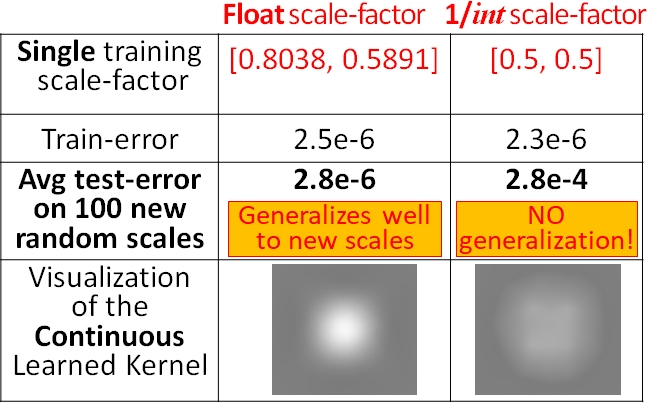
\includegraphics[width=1.1\textwidth]{figs/fig_generalize_Michal.jpg}
   \captionsetup{oneside, margin={-0.1cm,-0.2cm}}
  \captionof{figure}{\it  CC trained on one (float) scale, generalizes well to other scales.}
    \label{fig:generalize}
\end{minipage}

\end{minipage}


\textbf{The power of dynamic Scale-Ensembles at inference:}
%To demonstrate the potential use of CC-layers in image classification tasks, we did the following simple experiment:
Since \michal{the above} ``CC-Net'' was trained with non-integer (float) \michal{internal} scale-factors, it can generalize to new \michal{internal} scale-factors \emph{at inference-time}. This gives rise to \emph{ensemble-based image classification} (Sec.~\ref{sec:features} \& Fig.~\ref{fig:scale_ensemble}). 
This means that our trained CC-Net can be applied numerous times at inference, each time with a different sequence of scales (as long as their product yields 1/4), and average the \niv{logits}
% probabilities
of all forwarded passes.
%We tested this for 1,2,3 applications of CC-Net. Even small ensembles 
\michal{We tested this for CC-Net. Even small ensembles (2,3)}
already gave a significant boost in classification accuracy (+1.7\%, +2.4\%, respectively).
\michal{While test-time augmentations for regular CNNs can be applied  to the input image only, Scale-Ensembles apply test-time augmentation to \emph{all} CC-layers in the network. Hence, deep nets with many CC-layers, are likely to benefit from larger self-ensembles.}
%
% For reference, when providing Baseline-Net with test-time augmentations of the input images (mild scale variations and horizontal-flip) and averaging probabilities, the improvement was very mild 
% %we used mild random scaling (scale-factor between 1 and 1.1) and center-cropping of the input image. We observed that scaling hardly improves their results so we also used horizontal flips for both our test-augmentations and for the baselines.
% Such augmentations gave a slight improvement (up to +1.1\% for 2 augmentations), but not as significant as the scale-ensembles (+2.2\% for 5 ensembles). 

\textbf{Potential use in image-processing tasks:}
CC-layers could potentially be very useful in image-processing tasks. For example, existing Super-Resolution (SR) networks are trained for a fixed scale-factor~\cite{EDSR, srcnn}. To increase the resolution of an image by a factor of 3, one must use a SRx3 net which was trained for this specific scale-factor. SR by a factor of 4 will require a different pretrained SRx4  net. 
Constructing a SR network based on CC-layers is expected to give \emph{SR with any desired scale factor} (or at least an impressive range of scale-factors), all \emph{with a single trained SR net}. 
%Moreover, it should be able to accommodate different SR scale factors for different axes, if so desired.
\michal{Moreover, it could potentially accommodate different SR scale factors for different axes (if so desired). Note that training a separate net for every potential SR scale 
(or any combination of vertical~x~horizontal SR scales) 
is combinatorially daunting. A CC-based SR network may alleviate this problem.}
Designing such a CC-based SR network is part of our future work.
